\documentclass[a4paper,12pt]{article}
\documentclass[a4paper,11pt]{article}
\usepackage[utf8]{inputenc}
\usepackage[T1]{fontenc}
\usepackage[french]{babel}
\usepackage[ddmmyyyy]{datetime}
\usepackage[table]{xcolor}
\usepackage{lmodern,mathptmx,changepage,titlesec,hyperref,listings,lstautogobble,graphicx,array,longtable,multirow,lipsum,tikz,shorttoc,enumitem,float,verbatim, amsthm,amsfonts,amsmath,amssymb,mathrsfs,thmtools}
\usetikzlibrary{arrows,automata}
\usetikzlibrary{positioning}

\renewcommand{\rmdefault}{\sfdefault} %Utilisation de la police sans-serif ("Computer Modern Sans") pour la police roman
\renewcommand{\ttdefault}{pcr} 	%Utilisation d'une police "CourrierNew" pour la police monospaced (pour faire un listing manuel)
\linespread{1.15}				%Interligne

%Utilisation de liens colorés en bleu et soulignés
\hypersetup{colorlinks=true, urlcolor=blue, urlbordercolor=blue, linkcolor=black, linkbordercolor=white}
\makeatletter \Hy@AtBeginDocument{\def\@pdfborder{0 0 1} \def\@pdfborderstyle{/S/U/W 1}}\makeatother

\titlespacing*{\section} {0cm}{7ex plus 1ex minus .2ex}{1.5ex plus .2ex}
\titlespacing*{\subsection} {0cm}{4.5ex plus 1ex minus .2ex}{1.5ex plus .2ex}
\titleformat*{\section}{\huge\bfseries}
\titleformat*{\subsection}{\LARGE\bfseries}
\titleformat*{\subsubsection}{\normalsize\bfseries}

\definecolor{darkgreen}{rgb}{0.1,0.5,0.1}
\definecolor{mygray}{rgb}{0.93,0.93,0.93}
\definecolor{mymauve}{rgb}{0.58,0,0.82}
\lstset{	
	language=C,
	basicstyle=\small\ttfamily,
	backgroundcolor=\color{mygray},
	breaklines=true,
	breakatwhitespace=true,
	tabsize=3,
	captionpos=b,
	frame=none,
	rulecolor=\color{black},
	keywordstyle=\color{blue}\bfseries,
	stringstyle=\color{orange},
	showstringspaces=false,
	commentstyle=\footnotesize\color{darkgreen},
	keepspaces=true,
	extendedchars=true,
	numbers=left,
	numberstyle=\tiny\color{lightgray},
	stepnumber=1,
	escapeinside={(@}{@)},
	autogobble=true,
	literate=
		{á}{{\'a}}1 {é}{{\'e}}1 {í}{{}}1 {ó}{{\'o}}1 {ú}{{\'u}}1
		{Á}{{\'A}}1 {É}{{\'E}}1 {Í}{{\'I}}1 {Ó}{{\'O}}1 {Ú}{{\'U}}1
		{à}{{\`a}}1 {è}{{\`e}}1 {ì}{{\`i}}1 {ò}{{\`o}}1 {ù}{{\`u}}1
		{À}{{\`A}}1 {È}{{\'E}}1 {Ì}{{\`I}}1 {Ò}{{\`O}}1 {Ù}{{\`U}}1
		{ä}{{\"a}}1 {ë}{{\"e}}1 {ï}{{\"i}}1 {ö}{{\"o}}1 {ü}{{\"u}}1
		{Ä}{{\"A}}1 {Ë}{{\"E}}1 {Ï}{{\"I}}1 {Ö}{{\"O}}1 {Ü}{{\"U}}1
		{â}{{\^a}}1 {ê}{{\^e}}1 {î}{{\^i}}1 {ô}{{\^o}}1 {û}{{\^u}}1
		{Â}{{\^A}}1 {Ê}{{\^E}}1 {Î}{{\^I}}1 {Ô}{{\^O}}1 {Û}{{\^U}}1
		{œ}{{\oe}}1 {Œ}{{\OE}}1 {æ}{{\ae}}1 {Æ}{{\AE}}1 {ß}{{\ss}}1
		{ç}{{\c c}}1 {Ç}{{\c C}}1 {ø}{{\o}}1 {å}{{\r a}}1 {Å}{{\r A}}1
		{€}{{e}}1 {£}{{\pounds}}1 {«}{{\guillemotleft}}1
		{»}{{\guillemotright}}1 {ñ}{{\~n}}1 {Ñ}{{\~N}}1 {¿}{{?`}}1
}

\lstdefinestyle{terminal}{
	language=bash,
	backgroundcolor=\color{black},
	basicstyle=\color{white}\small\ttfamily
}

%Redéfinition de la taille de \Huge pour le titre du document
\makeatletter\renewcommand\Huge{\@setfontsize\Huge{37pt}{40}}\makeatother
\date{\today}
\setlength{\parindent}{0pt}
\usepackage[right=3.2cm, left=3.2cm, bottom=3.5cm, top=3cm, footskip=1.5cm,]{geometry}

\title{\textbf{Programmation système}}
\author{
	Steve Alabi - Taha Bendjeddou - Younes Benyamna - Malek Zemni
	\vspace{1em}\\
	Feuille d'exercices
	\vspace{0.5em}
}
\linespread{1.35}	

\begin{document}
\maketitle

	\subsection*{Exercice 1} 
	\textit{(définitions générales, gestion de flux et entrées / sorties)}
	\\~\\
	1/ Définir précisément un appel-système. Comment s'exécutent-ils ?\\ 
	2/ En quoi la redirection de flux peut-elle servir dans la gestion d'erreurs ? \\
	3/ Écrire une fonction \lstinline!myGetChar! analogue à la fonction \lstinline!fgetc! (lecture d'un seul caractère à partir d'un fichier) en utilisant uniquement des appels-systèmes.\\
	4.1/ Définir un buffer. \\
	4.2/ Expliquer comment construire une version bufferisée de la fonction \lstinline!myGetChar!.\\
	4.3/ Écrire la fonction \lstinline!myGetChar! bufferisée.
	
	\subsection*{Exercice 2} 
	\textit{(processus)}
	\\~\\
	1/ Quelle est la particularité des processus sous les systèmes UNIX ?\\
	2/ Donner une légende correspondant aux numéros (1, 2, 3 et 4) de la figure suivante :
	\begin{center}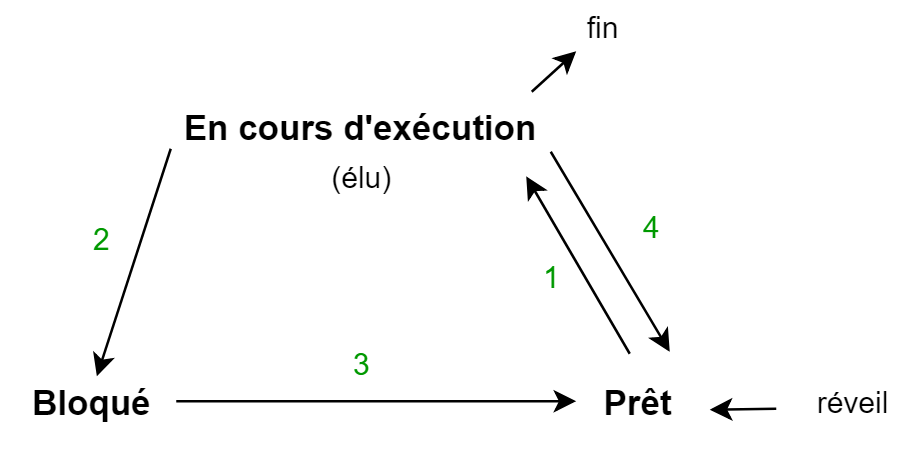
\includegraphics[scale=0.4]{../img/process.png}\end{center}
	3/ Définir un processus zombie. Quelle est l'utilité de la fonction \lstinline!wait! ?\\
	4/ Lors de la création d'un nouveau processus, quelles ressources sont dupliquées et lesquelles sont partagées ?\\
	5/ Écrire un programme qui crée un processus et qui affiche un message différents pour chaque processus (en incluant la gestion d'erreurs). 
	
	\subsection*{Exercice 3} 
	\textit{(threads)}
	\\~\\
	1/ Quelle est la différence entre un processus et un thread ? Quel est l'avantage des threads ?\\
	2/ Écrire un programme ayant le comportement suivant :
	\begin{itemize}
		\item des threads sont créés (leur nombre étant passé en paramètre lors du lancement du programme)
		\item chaque thread affiche un message (par exemple "hello world !") et son PID
		\item le thread principal attend la terminaison des différents threads créés
	\end{itemize}
	3/ Définir un mutex et donner son rôle.\\
	4/ Écrire un programme qui crée deux threads : un qui incrémente une variable compteur par un nombre tiré au hasard entre 0 et 10, et l'autre qui affiche un message lorsque la variable compteur dépasse 20 (utiliser mutex et conditions).
\end{document}